\section{Campagnes de mesure}
\label{sec:mesures}

\begin{resume}
Le multic\oe{}ur apporte $+8$ \`a $+26\,\%$ de simulations par seconde selon la
position, avec un plafond d\`es deux workers et un p95 de latence qui ne se
d\'egrade pas. La comparaison interleaved avec l'ancien binaire ne montre
aucune r\'egression mono-worker. Le self-play partage reste identique au bit
pr\`es sur ses compteurs et ses visites. La qualit\'e est non inf\'erieure sur
2\,500 puzzles (delta $-0,28$ point, IC95 $[-0,8\,;+0,24]$), et le test \`a
temps \'egal se conclut \`a une \'egalit\'e (364 contre 366). La mesure du
r\'egime r\'eel du bot montre que la tranche de 64 simulations utilis\'ee par
la boucle UCI est le r\'egime favorable, alors que la tranche de 8 du banc
p\'enalise artificiellement huit workers. Le r\'eglage
\code{MCTS\_WORKER\_COUNT = 8} est activ\'e.
\end{resume}

\subsection{Protocole et mat\'eriel}

Toutes les campagnes utilisent le m\^eme mod\`ele
(\chemin{2026\_04\_23\_23h25\_iter316\_unsupervised.onnx}, sha256
\code{20a19f82e170}), la m\^eme politique \code{h0}, une table de
8\,192 entr\'ees, un lot de 8 et $c_{\text{puct}} = 1{,}4$. La machine est un
portable RTX PRO 2000 Blackwell (8\,Gio, driver 595.95) avec un CPU de
16 c\oe{}urs logiques (Intel64 Family 6 Model 197). ONNX Runtime 1.24.3
utilise le provider CUDA. Les trois positions de r\'ef\'erence sont
l'ouverture, le milieu et la finale, d\'efinies en annexe~C.

\begin{mesure}[Le protocole de d\'ebit]
Chaque configuration est mesur\'ee 30 fois (campagne principale,
$5 \times 6$ passages) ou 50 fois (campagne de queue), en alternant l'ordre
des workers \`a chaque passage pour que la d\'erive thermique se r\'epartisse
\'equitablement. Le mode \code{--warmup-pool} conserve l'objet MCTS entre les
mesures et remet arbre et table \`a froid hors chronom\'etrage, de sorte que
les m\'edianes d\'ecrivent le r\'egime \'etabli et que le premier appel de
chaque configuration (cr\'eation des threads, premi\`ere passe) soit mesur\'e
s\'epar\'ement. Les sessions varient de 15 \`a 30\,\% entre elles : seules les
comparaisons intra-session sont utilis\'ees pour conclure.
\end{mesure}

\subsection{Aucune r\'egression mono-worker}

Comparer le nouveau moteur \`a l'ancien pose un probl\`eme pratique : le
binaire d'avant n'existe plus. Le pyd de l'\'epoque (commit \code{da29e7b})
\'etait committ\'e dans Git ; il a \'et\'e extrait dans un r\'epertoire
temporaire,
le banc actuel y a \'et\'e copi\'e avec un repli \code{TypeError} pour
l'appel sans \code{worker\_count}, et les deux moteurs ont \'et\'e mesur\'es
en alternance, trois rounds de trois passages. L'alternance est essentielle :
l'ancien moteur fluctue de 700 \`a 1\,200 simulations par seconde selon
l'\'etat d'horloge du GPU, contre 700 \`a 820 pour le nouveau. Les rounds 1
et 2 donnent des rapports nouveau/ancien de 0,97 \`a 1,14 ; le round 3 est un
pic de boost de l'ancien (1\,018 sims/s en ouverture) que le nouveau ne
suit pas, sans que cela traduise une r\'egression. Les compteurs et les
distributions de visites sont identiques. Conclusion : pas de r\'egression
d'infrastructure visible en mono-worker, ce qui \'etait la condition pour
interpr\'eter le gain multic\oe{}ur.

\subsection{D\'ebit et latence par nombre de workers}

La campagne principale donne les m\'edianes de la figure et du tableau
suivants (chemin \code{step\_analysis}, pool chaud, 30 observations).

\begin{figure}[t]
\centering
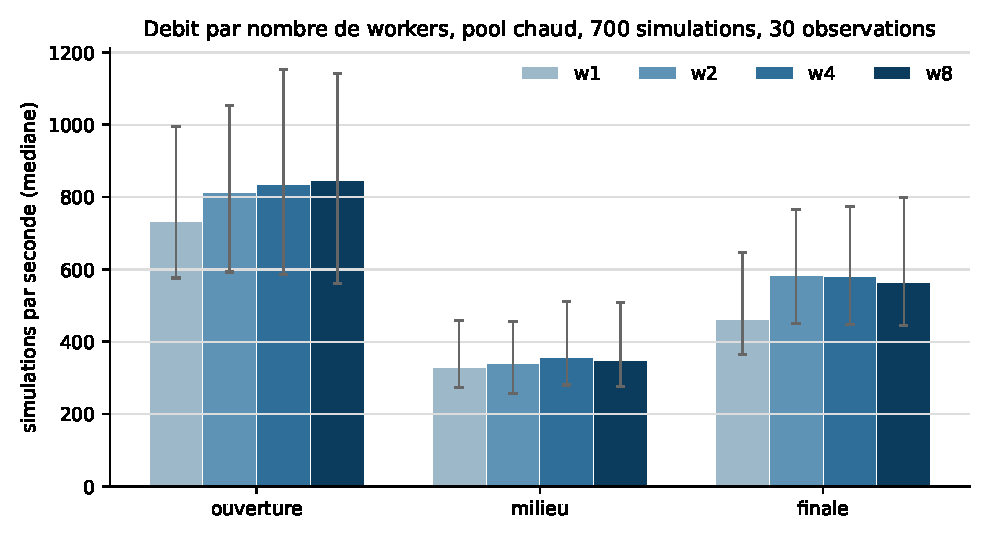
\includegraphics[width=0.86\textwidth]{figures/fig_debit_workers.pdf}
\caption{M\'edianes de d\'ebit par position et par nombre de workers, pool
chaud, 700 simulations, 30 observations par point (\code{after.json}). Les
barres d'erreur vont du minimum au maximum observ\'e.}
\label{fig:debit}
\end{figure}

\begin{center}
\small
\begin{tabular}{lccccr}
\toprule
Position & w1 & w2 & w4 & w8 & gain w8 \\
\midrule
ouverture & 733,5 & 812,3 & 835,0 & 846,8 & $+15{,}4\,\%$ \\
milieu    & 328,7 & 340,7 & 356,1 & 348,8 & $+6{,}1\,\%$ \\
finale    & 462,2 & 583,8 & 579,2 & 565,1 & $+22{,}3\,\%$ \\
\bottomrule
\end{tabular}
\captionof{table}{M\'edianes de simulations par seconde,
\code{step\_analysis}, pool chaud. Le gain plafonne d\`es deux workers ;
\code{mcts\_search} donne les m\^emes ordres.}
\label{tab:debit}
\end{center}

La campagne de queue, avec 50 observations par configuration et deux
configurations seulement (1, 2 et 8 workers), confirme ces ordres de grandeur
et permet de mesurer proprement la distribution.

\begin{piege}[Le p95 de latence n'est pas le p95 de d\'ebit]
Le crit\`ere d'acceptation porte sur la \emph{latence} d'une recherche de
700 simulations. Or la latence est l'inverse du d\'ebit : le p95 de latence
correspond au \emph{p5} du d\'ebit, c'est-\`a-dire aux recherches les plus
lentes. Comparer le p95 du d\'ebit d'une configuration \`a celui d'une autre
mesure la mauvaise queue, et donne l'impression inverse : on croit voir une
d\'egradation alors que les recherches lentes s'am\'elioreraient. Le rapport
de latence vaut $L_{95}(w_8)/L_{95}(w_1) = p_5(T_{w_1})/p_5(T_{w_8})$.
\end{piege}

\begin{figure}[t]
\centering
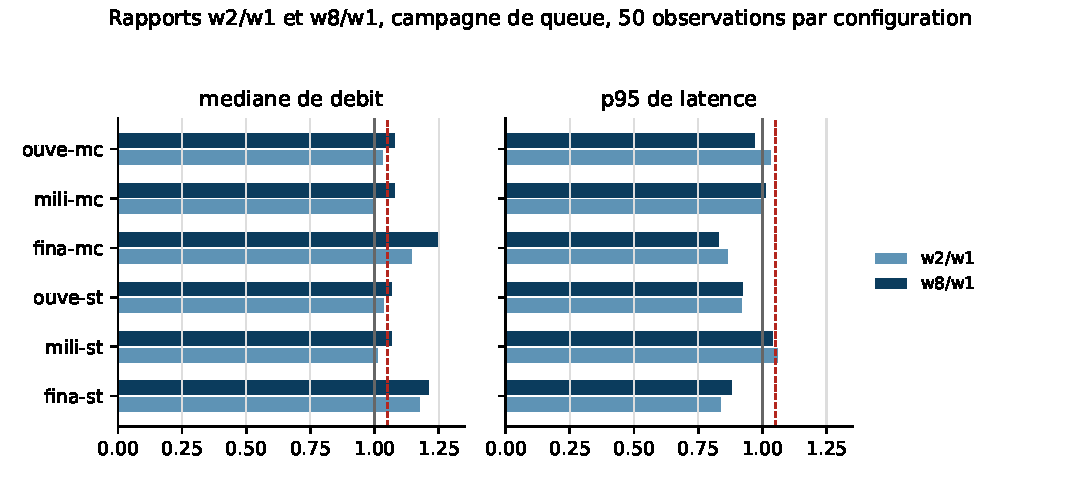
\includegraphics[width=0.86\textwidth]{figures/fig_queue_latence.pdf}
\caption{Rapports w2/w1 et w8/w1 sur la campagne de queue (50 observations
par configuration) : m\'ediane de d\'ebit et p95 de latence. En dessous de la
ligne des 5\,\%, le crit\`ere est franchi.}
\label{fig:queue}
\end{figure}

Avec la bonne d\'efinition, w8 franchit le crit\`ere partout : rapports de
p95 de latence de 0,832 \`a 1,045 selon les six couples position-chemin, tous
sous $+5\,\%$, et m\^eme am\'elior\'es sur la finale ($-12$ \`a $-17\,\%$).
w2 franchit le crit\`ere partout sauf un point marginal (milieu
\code{step\_analysis}, $+6{,}4\,\%$), et capture d\'ej\`a l'essentiel du gain
de m\'ediane. Le candidat retenu reste w8, qui a les meilleures m\'edianes
globales et la queue la plus stable.

\subsection{R\'epartition par phase et remplissage}

La campagne \`a chronom\'etrages actifs (3 mesures par configuration) montre
que l'inf\'erence occupe 96,6 \`a 98,7\,\% du temps mur, dans toutes les
configurations. En huit workers, l'attente de barri\`ere ne p\`ese que 1,5 \`a
2,3\,\% : 24,3\,ms en finale, 40,7\,ms en milieu, 19,3\,ms en ouverture pour
des recherches de 1,3 \`a 2,3 secondes.

\begin{figure}[t]
\centering
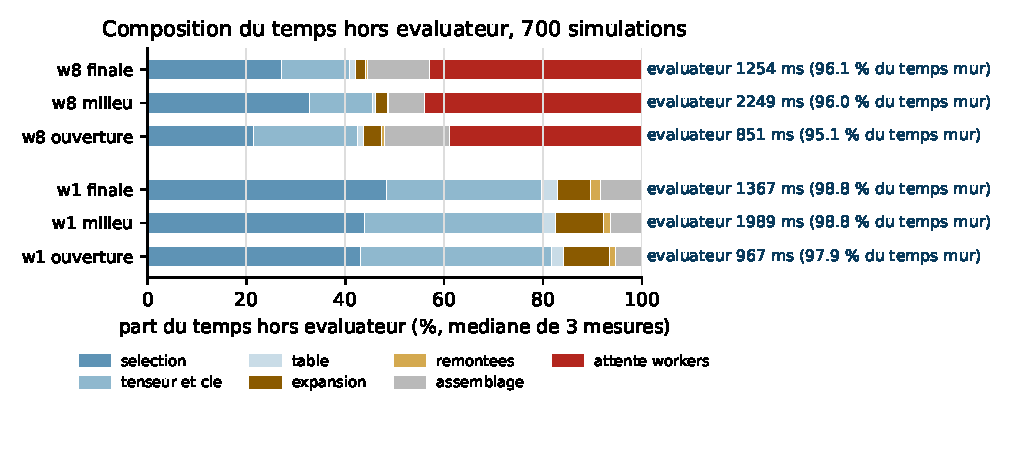
\includegraphics[width=0.86\textwidth]{figures/fig_phases.pdf}
\caption{Part du temps mur consacr\'ee \`a l'inf\'erence et au reste (somme
des phases CPU et de l'attente), par position, en w1 et w8. Le reste est
d\'ej\`a minuscule en w1 ; le multic\oe{}ur le r\'eduit encore, mais ne peut
pas toucher \`a l'inf\'erence.}
\label{fig:phases}
\end{figure}

Le remplissage progresse l\'eg\`erement : de 6,1 \`a 6,7 en finale et de 6,9
\`a 7,2 en ouverture. Cette hausse r\'eduit le nombre d'appels GPU physiques
pour un m\^eme nombre de positions, ce qui est une part du gain mesur\'e :
le multic\oe{}ur ne fait pas que parall\'eliser la collecte, il ferme moins
souvent des lots partiels.

\subsection{Le r\'egime r\'eel de la boucle UCI}

Le bot n'appelle pas \code{step\_analysis} une fois pour 700 simulations : sa
boucle avance par tranches de \code{BATCH\_SIZE = 64} simulations, sur un
arbre et un pool persistants. Un diagnostic d\'edi\'e a mesur\'e ce
r\'egime, avec des tranches de 64 et de 20, sur 704 simulations et trois
r\'ep\'etitions.

\begin{center}
\small
\begin{tabular}{llccr}
\toprule
Tranche & Position & w1 (sims/s) & w8 (sims/s) & gain \\
\midrule
64 & ouverture & 799,1 & 912,5 & $+14\,\%$ \\
64 & milieu    & 373,1 & 462,8 & $+24\,\%$ \\
64 & finale   & 582,5 & 580,0 & $0\,\%$ \\
20 & ouverture & 503,9 & 572,4 & $+14\,\%$ \\
20 & milieu    & 244,5 & 256,1 & $+5\,\%$ \\
20 & finale   & 319,1 & 405,5 & $+27\,\%$ \\
\bottomrule
\end{tabular}
\captionof{table}{R\'egime r\'eel du bot : \code{step\_analysis} r\'ep\'et\'e
par tranches, arbre et pool persistants, 704 simulations, 3 r\'ep\'etitions.}
\label{tab:tranches}
\end{center}

\begin{figure}[t]
\centering
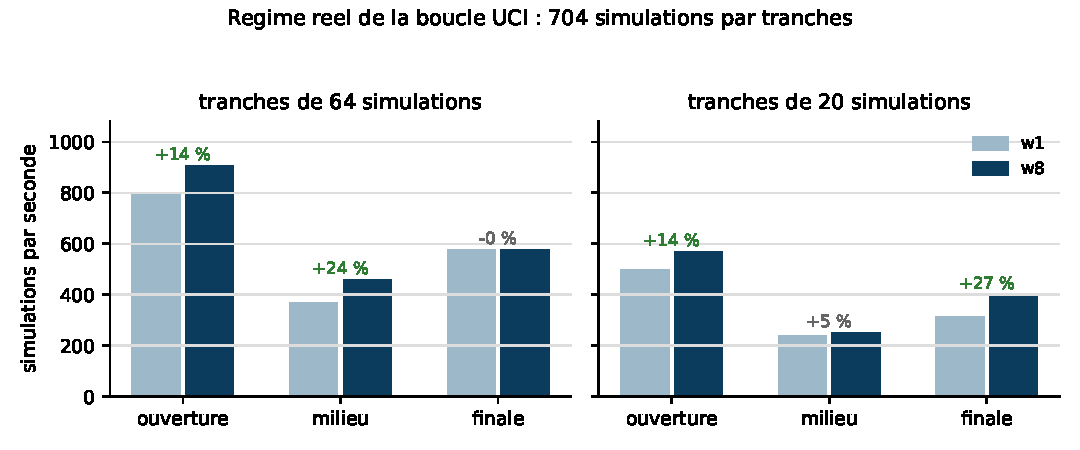
\includegraphics[width=0.78\textwidth]{figures/fig_tranches_uci.pdf}
\caption{Gain de w8 par rapport \`a w1 selon la taille de tranche. Aux deux
tranches du bot (64 et 20 simulations), le gain est net sauf en finale \`a 64 ;
\`a 8, non repr\'esent\'e ici, les arbres naissants font exploser les collisions
et w8 recule.}
\label{fig:tranches}
\end{figure}

\`A la tranche de 8 simulations (celle du protocole \`a temps \'egal du banc
puzzle), le rapport s'inverse : w8 tombe \`a 693 sims/s contre 857 pour w1,
avec 970 collisions pour 800 simulations. Un arbre de huit simulations est
trop jeune pour offrir huit branches distinctes ; les workers se disputent
les quelques feuilles existantes, et le co\^ut des collisions d\'epasse le
gain de parall\'elisme. Ce ph\'enom\`ene n'existe plus \`a 64 simulations :
la phase la plus jeune de chaque recherche est courte relativement au budget,
et les collisions, bien que nombreuses (1\,300 \`a 3\,300 par 704
simulations), sont amorties. C'est le r\'egime du bot, et c'est celui qui
compte.

\subsection{Non-r\'egression du self-play}

Le banc \code{selfplay\_phase\_bench} a \'et\'e rejou\'e avec les m\^emes
r\'eglages que la r\'ef\'erence de la t\^ache~2 : huit plateaux, 100 vagues,
30 r\'epetitions.

\begin{center}
\small
\begin{tabular}{llrrl}
\toprule
Variante & Mesure & Avant & Apr\`es & Rapport \\
\midrule
fake & collecte & 0,738 ms & 1,321 ms & $+79\,\%$ \\
fake & traitement & 4,390 ms & 4,508 ms & $+2{,}7\,\%$ \\
GPU  & collecte & 1,928 ms & 2,003 ms & $+3{,}9\,\%$ \\
GPU  & traitement & 340,97 ms & 305,04 ms & $-10{,}5\,\%$ \\
\bottomrule
\end{tabular}
\captionof{table}{Banc self-play partag\'e, m\'edianes de 30 r\'epetitions.
Les compteurs (800 appels, 100 lots, 103 succ\`es de table en GPU) et les
visites de r\'ef\'erence sont identiques avant et apr\`es.}
\label{tab:selfplay}
\end{center}

Le surco\^ut CPU des nouveaux \'etats atomiques, du cache et des
r\'eservations vaut environ 0,58\,ms pour 100 vagues en mode fake, soit
5,8 microsecondes par vague. Il est visible en relatif parce que le faux
r\'eseau ne co\^ute rien, et n\'egligeable en absolu face aux 305\,ms de
r\'eseau en GPU. Le traitement GPU mesur\'e est m\^eme plus rapide
apr\`es qu'avant, ce qui rel\`eve de l'\'etat d'horloge de la session, pas du
chantier : l'important est que les compteurs et les visites soient
identiques au bit pr\`es, ce qui prouve que la s\'emantique du self-play est
intacte.

\subsection{Qualit\'e de recherche}

La qualit\'e est mesur\'ee sur le banc de puzzles, au premier coup, avec le
crit\`ere fig\'e \code{reussi\_recherche}. Trois campagnes ont \'et\'e
men\'ees, toutes sur GPU, un seul processus, avec comparaison appari\'ee et
bootstrap \`a 20\,000 tirages (seed 42).

\begin{figure}[t]
\centering
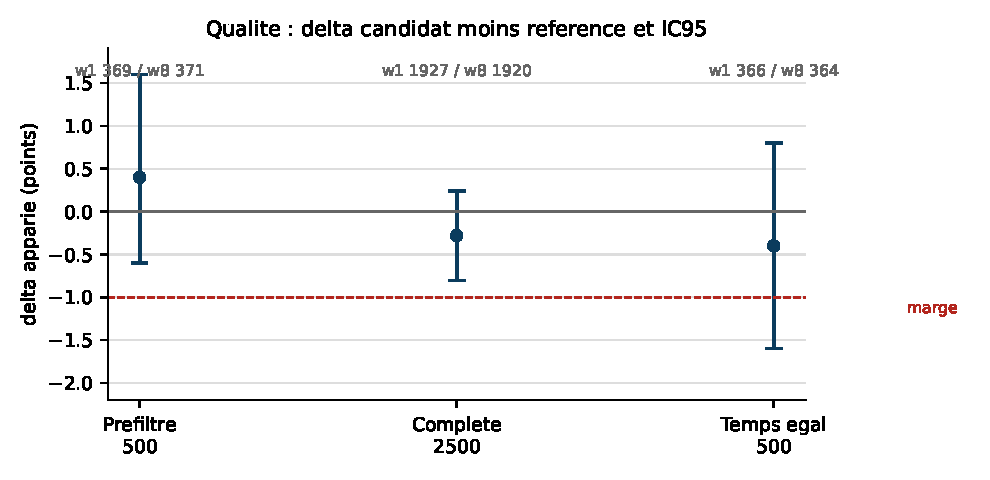
\includegraphics[width=0.86\textwidth]{figures/fig_qualite.pdf}
\caption{Taux de r\'esolution et intervalles de confiance bootstrap pour les
trois campagnes. La ligne pointill\'ee marque la marge de non-inf\'eriorit\'e
de $-1$ point sur l'intervalle du delta appari\'e.}
\label{fig:qualite}
\end{figure}

\begin{center}
\small
\begin{tabular}{llrrl}
\toprule
Campagne & n & w1 & w8 & delta appari\'e (IC95) \\
\midrule
Pr\'efiltre (700 sims) & 500 & 369 & 371 &
$+0{,}4$ pt $[-0{,}6\,;+1{,}6]$ \\
Complete (700 sims) & 2\,500 & 1\,927 & 1\,920 &
$-0{,}28$ pt $[-0{,}8\,;+0{,}24]$ \\
Temps \'egal (1,5 s) & 500 & 366 & 364 &
$-0{,}4$ pt $[-1{,}6\,;+0{,}8]$ \\
\bottomrule
\end{tabular}
\captionof{table}{Qualit\'e : r\'eussites et delta candidat moins
r\'ef\'erence. Seule la campagne \`a simulations \'egales sert au verdict de
non-inf\'eriorit\'e ; le test \`a temps \'egal quantifie le gain pratique.}
\label{tab:qualite}
\end{center}

Trois lectures. D'abord, la campagne compl\`ete \`a 2\,500 puzzles donne un
delta de $-0,28$ point, avec vingt-quatre paires perdues contre dix-sept
gagn\'ees et un McNemar non significatif ($p = 0{,}35$). La borne basse
$-0{,}8$ point est \`a l'int\'erieur de la marge de $-1$ point : le verdict
formel est la non-inf\'eriorit\'e. Par tranche de rating, les deltas vont de
$-0{,}16$ \`a $-0{,}48$ point, sans concentration : c'est du bruit sur
l'\'echantillon, pas un effet localis\'e. Ensuite, la r\'ep\'etition du
candidat prescrite par le plan en cas d'intervalle proche du seuil a \'et\'e
\'ecart\'ee par le propri\'etaire pour des raisons de dur\'ee : c'est la
r\'eserve principale de ce verdict. Enfin, la mesure \`a temps \'egal,
avec un budget de 1,5 seconde par puzzle (la m\'ediane observ\'ee des 700
simulations mono-worker), donne une \'egalit\'e : 364 contre 366, intervalle
$[-1{,}6\,;+0{,}8]$, ind\'etermin\'e. Huit workers y terminent 472
simulations m\'edianes contre 728, pour la raison m\'ecanique d\'ecrite au
chapitre~6.5 : le protocole \`a tranches de 8 p\'enalise les arbres naissants.
Le taux de r\'esolution, lui, reste \'egal. Le d\'epassement du dernier
appel complet, en mode temps, a une m\'ediane de 8,8\,ms et un p95 de
51\,ms, ce qui est tr\`es inf\'erieur \`a la granularit\'e d'une tranche.

\subsection{La d\'ecision d'activation}

Tous les crit\`eres du plan sont franchis : m\'ediane am\'elior\'ee de
fa\c{c}on reproductible, p95 de latence sous $+5\,\%$ partout, invariants
v\'erifi\'es, non-inf\'eriorit\'e qualit\'e au seuil pr\`es, self-play
identique. Le r\'eglage \code{MCTS\_WORKER\_COUNT = 8} a donc \'et\'e ajout\'e
\`a c\^ot\'e de \code{MCTS\_BATCH\_SIZE = 8} dans \code{uci.py}, avec un test
de transmission qui v\'erifie le cinqui\`eme argument r\'eel de
\code{step\_analysis}, et un smoke UCI complet en sous-processus. Les
r\'eserves sont list\'ees au chapitre~7.
